\documentclass[a4paper,12pt]{article}
\usepackage[utf8]{inputenc}
\usepackage{tikz}
\usetikzlibrary{automata,positioning}
\usepackage{amssymb}
\usepackage{hyperref}
\hypersetup{
	unicode=true,         	% non-Latin characters in Acrobat�s bookmarks
	pdftoolbar=true,        % show Acrobat�s toolbar?
	pdfmenubar=true,        % show Acrobat�s menu?
	pdffitwindow=false,     % window fit to page when opened
	pdfstartview={FitH},    % fits the width of the page to the window
	pdftitle={Projet : Compilateur Perl},  
    pdfauthor={Rodriguez Paul, Vaccari Eric},	
    pdfnewwindow=true,      % links in new window
    colorlinks=true,       % false: boxed links; true: colored links
    linkcolor=black,          % color of internal links
    citecolor=green,        % color of links to bibliography
    filecolor=magenta,      % color of file links
    urlcolor=cyan           % color of external links
}
\begin{document}
	\begin{center}
		\begin{huge}\textbf{INFO-F-403}\end{huge}\\ 
		\bigskip \bigskip
		\begin{Huge}\textbf{Projet : Compilateur Perl}\end{Huge}\\
		
		\vspace*{9cm}
		\begin{Large}
		\textbf{Auteurs :}
		\vspace{0,1cm}
		\vspace{0,5cm}
			\bigskip \bigskip \bigskip 
			\begin{tabular}{l@{\hspace*{1,2cm}} l@{\vspace*{0,3cm}}}			
				Rodriguez Paul\\
				Vaccari Eric\\
			\end{tabular} 
		\end{Large}
	\end{center}

\section{Unités lexicales}
	\subsection{Tableau}
		\begin{center}
		    \begin{tabular}{ | l | l |}
		    	\hline Nom & Regex \\
		    	\hline var & \verb@ $[a-zA-Z_][a-zA-Z0-9_]* @ \\
		    	\hline identifier & \verb@ [a-zA-Z_][a-zA-Z0-9_]* @ \\
		    	\hline integer & \verb@ [0-9]+ @ \\
		    	\hline float & \verb@ {integer}\.{integer} @ \\
		    	\hline string & \verb@ '[^']*' @ \\
		    	\hline space & \verb@ [\t\n ] @ \\
		    	\hline comment & \verb@ #.*\n @ \\
		    	\hline lbrace & \verb@ \{ @ \\
		    	\hline rbrace & \verb@ \} @ \\
		    	\hline lpar & \verb@ \( @ \\
		    	\hline rpar & \verb@ \) @ \\
		    	\hline semicolon & \verb@ ; @ \\
		    	\hline call\_mark & \verb@ & @ \\
		    	\hline plus & \verb@ \+ @ \\
		    	\hline minus & \verb@ \- @ \\
		    	\hline times & \verb@ \* @ \\
		    	\hline divide & \verb@ \/ @ \\
		    	\hline not & \verb@ ! @ \\
		    	\hline notletters & \verb@ not @ \\
		    	\hline lazy\_and & \verb@ && @ \\
		    	\hline lazy\_or & \verb@ || @ \\
		    	\hline equals & \verb@ == @ \\
		    	\hline eq & \verb@ eq @ \\
		    	\hline different & \verb@ != @ \\
		    	\hline ne & \verb@ ne @ \\
		    	\hline lower & \verb@ < @ \\
		    	\hline lt & \verb@ lt @ \\
		    	\hline greater & \verb@ > @ \\
		    	\hline gt & \verb@ gt @ \\
		    	\hline lower\_equals & \verb@ <= @ \\
		    	\hline le & \verb@ le @ \\
		    	\hline greater\_equals & \verb@ >= @ \\
		    	\hline ge & \verb@ ge @ \\
		    	\hline comma & \verb@ , @ \\
		    	\hline concat\_mark & \verb@ \. @ \\
		    	\hline assign\_mark & \verb@ = @ \\
		    	\hline
			\end{tabular}	

			\begin{tabular}{ | l | l |}
				\hline Nom & Regex \\
		    	\hline sub & \verb@ sub @ \\
		    	\hline if & \verb@ if @ \\
		    	\hline else & \verb@ else @ \\
		    	\hline elseif & \verb@ elseif @ \\
		    	\hline unless & \verb@ unless @ \\
		    	\hline return & \verb@ return @ \\
		    	\hline defined & \verb@ defined @ \\
		    	\hline int & \verb@ int @ \\
		    	\hline length & \verb@ length @ \\
		    	\hline print & \verb@ print @ \\
		    	\hline scalar & \verb@ scalar @ \\
		    	\hline substr & \verb@ substr @ \\
		    	\hline
		    \end{tabular}
		\end{center}
	
	\subsection{Remarques}
		La syntaxe complète de Perl concernant les noms de variables est beaucoup plus
		compliquée mais concerne des fonctionalités (packages) hors du cadre de ce
		projet, ce pourquoi nous nous sommes limités aux règles les plus simples.
	
\section{Graphe du DFA}

	\subsection{Variables, comparateurs, blocs, litéraux}
		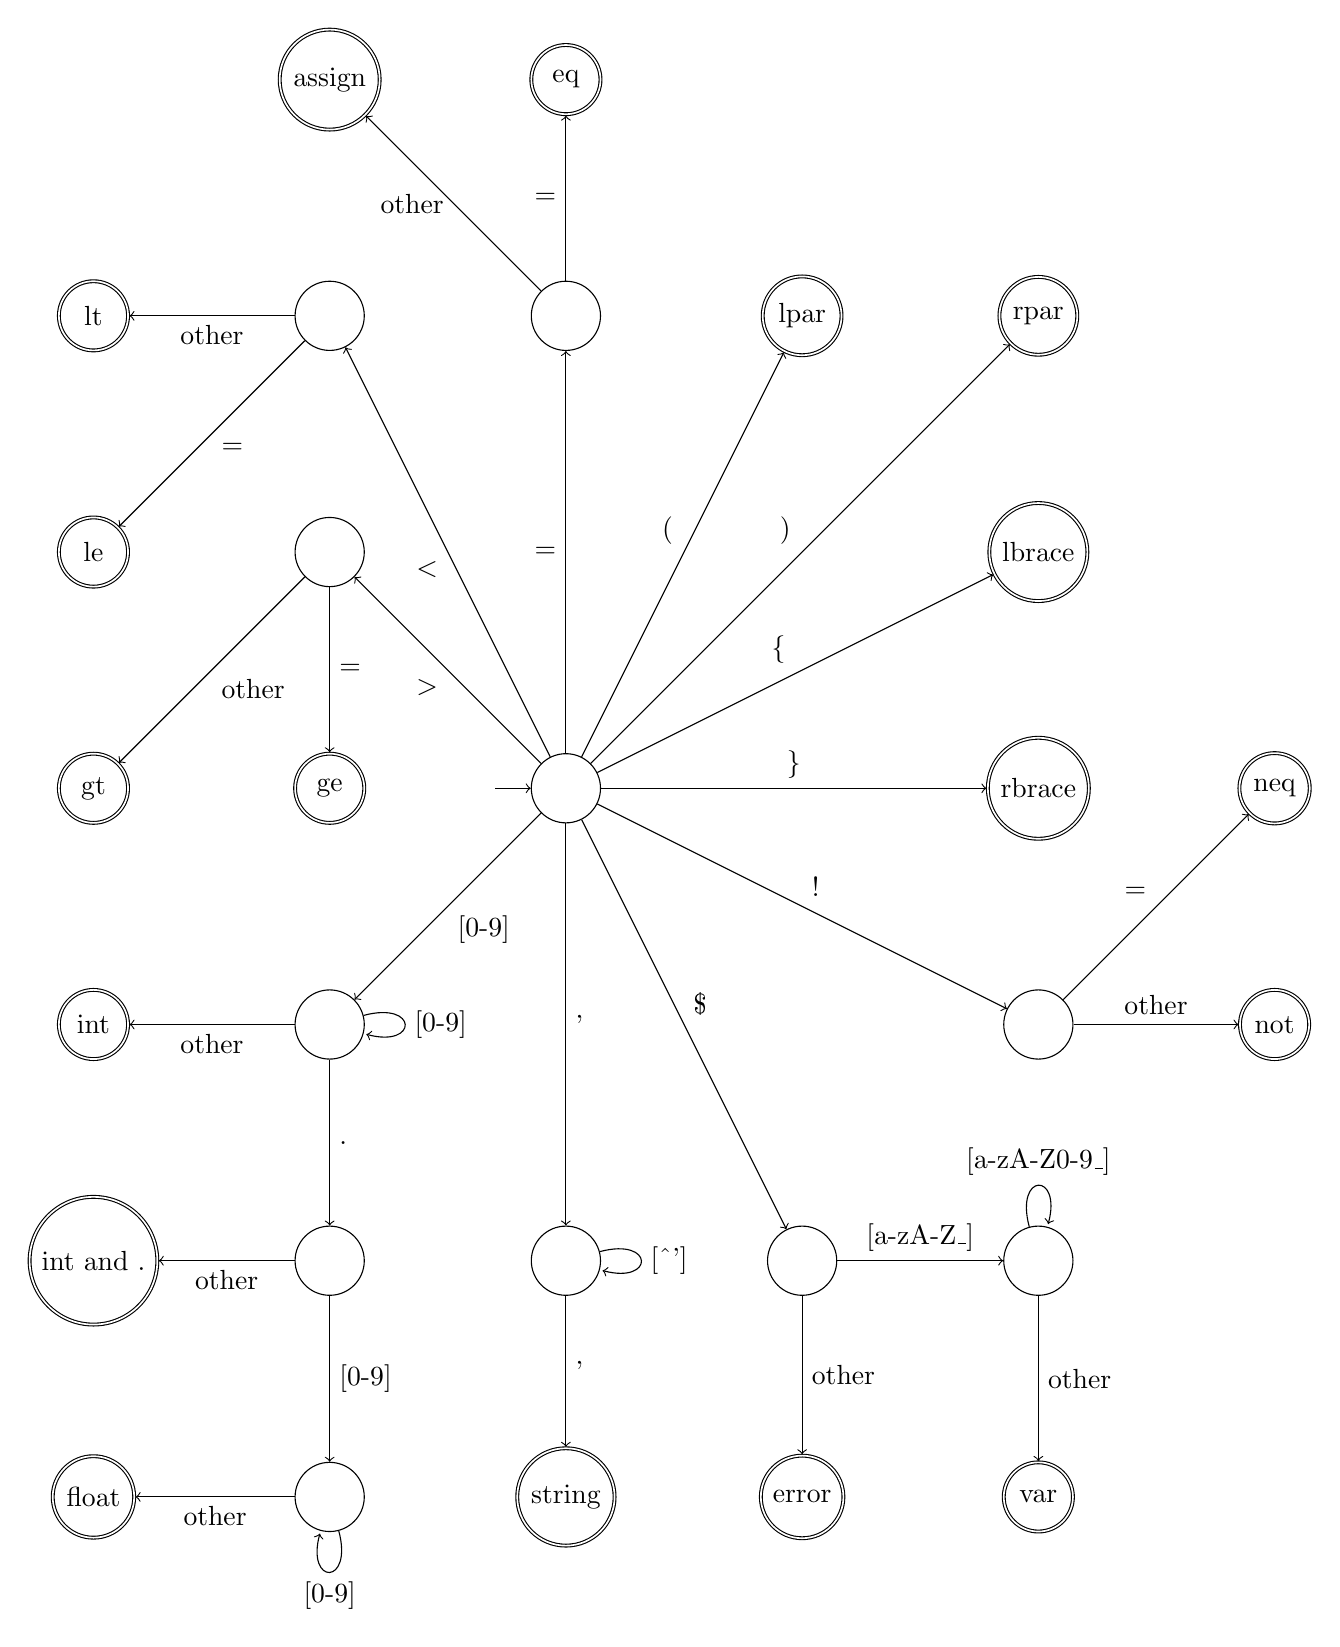
\begin{tikzpicture}[node distance=3cm,on grid,auto]
			\node[initial,initial text=,state] (0) {};
			\node[state] (6) [below=6cm of 0] {};
				\path[->] (0) edge node {'} (6);
				\path[->] (6) edge[loop right] node {[\^{}']} (6);
			\node[state] (1) [right of=6] {};
				\path[->] (0) edge node {\$} (1);
			\node[state,accepting] (11) [below of=1] {error};
				\path[->] (1) edge node{other} (11);
			\node[state] (5) [right of=1] {};
				\path[->] (1) edge node {[a-zA-Z\_]} (5);
				\path[->] (5) edge[loop above] node {[a-zA-Z0-9\_]} (5);
			\node[state,accepting] (12) [below of=5] {var};
				\path[->] (5) edge node{other} (12);
			\node[state,accepting] (7) [below of=6] {string};
				\path[->] (6) edge node{'} (7);
			\node[state] (3) [left of=6] {};
			\node[state] (2) [above of=3] {};
				\path[->] (0) edge node {[0-9]} (2);
				\path[->] (2) edge[loop right] node {[0-9]} (2);
			\node[state,accepting] (10) [left of=2] {int};
				\path[->] (2) edge node{other} (10);
				\path[->] (2) edge node {.} (3);
			\node[state,accepting] (8) [left of=3] {int and .};
				\path[->] (3) edge node{other} (8);
			\node[state] (4) [below of=3] {};
				\path[->] (3) edge node{[0-9]} (4);
				\path[->] (4) edge[loop below] node {[0-9]} (4);
			\node[state,accepting] (9) [left of=4] {float};
				\path[->] (4) edge node{other} (9);
			\node[state,accepting] (15) [left of=0] {ge};
			\node[state] (14) [above of=15] {};
				\path[->] (0) edge node{$>$} (14);
				\path[->] (14) edge node{=} (15);
			\node[state,accepting] (16) [left of=15] {gt};
				\path[->] (14) edge node{other} (16);
			\node[state] (13) [above of=14] {};
				\path[->] (0) edge node{$<$} (13);
			\node[state,accepting] (18) [left of=13] {lt};
				\path[->] (13) edge node{other} (18);
			\node[state,accepting] (17) [below of=18] {le};
				\path[->] (13) edge node{=} (17);
			\node[state] (19) [right of=13] {};
				\path[->] (0) edge node{=} (19);
			\node[state,accepting] (20) [above of=19] {eq};
				\path[->] (19) edge node{=} (20); 
			\node[state,accepting] (21) [left of=20] {assign};
				\path[->] (19) edge node[left]{other} (21);
			\node[state,accepting] (22) [right of=19] {lpar};
				\path[->] (0) edge node{(} (22);
			\node[state,accepting] (23) [right of=22] {rpar};
				\path[->] (0) edge node{)} (23);
			\node[state,accepting] (24) [below of=23] {lbrace};
				\path[->] (0) edge node{\{} (24);
			\node[state,accepting] (25) [below of=24] {rbrace};
				\path[->] (0) edge node{\}} (25);
			\node[state] (26) [below of=25] {};
				\path[->] (0) edge node{!} (26);
			\node[state,accepting] (27) [right of=26] {not};
				\path[->] (26) edge node{other} (27);
			\node[state,accepting] (28) [above of=27] {neq};
				\path[->] (26) edge node{=} (28);
		\end{tikzpicture}
		
	\subsection{Remarques}
		Le graphe a été scindé pour améliorer la clarté de l'ensemble.
		Certains tokens sont identifiables dés que leur dernier caractère a été lu (par exemple les accolades), 
		d'autres nécessitent la lecture du caractère suivant le dernier (par exemple, pour terminer un entier il faut lire autre chose qu'un chiffre).
		Dans ce deuxième cas, après avoir identifié le token la lecture du dernier caractère est annulée, il servira comme premier caractère du token suivant.


\end{document}